\documentclass[conference]{IEEEtran}
\IEEEoverridecommandlockouts
% The preceding line is only needed to identify funding in the first footnote. If that is unneeded, please comment it out.
\usepackage{cite}
\usepackage{amsmath,amssymb,amsfonts}
\usepackage{algorithmic}
\usepackage{float}
\usepackage{graphicx}
\usepackage{textcomp}
\usepackage{xcolor}
\def\BibTeX{{\rm B\kern-.05em{\sc i\kern-.025em b}\kern-.08em
    T\kern-.1667em\lower.7ex\hbox{E}\kern-.125emX}}

\DeclareGraphicsExtensions{.png,.PNG,.tiff,.tif,.jpeg,.jpg,.JPG,.JPEG,.gif}
\graphicspath{ {./images/} }

\begin{document}
\title{Software Defined Radio and it's use cases
}

\author{\IEEEauthorblockN{1\textsuperscript{st} Julian Janisch}
	\IEEEauthorblockA{\textit{Mobile Computing} \\
		\textit{FH OÖ Campus Hagenberg}\\
		Hagenberg im Mühlkreis, Österreich \\
		s1710237010@students.fh-hagenberg.at}
	\and
	\IEEEauthorblockN{2\textsuperscript{nd} Alexander Kemptner}
	\IEEEauthorblockA{\textit{Mobile Computing} \\
		\textit{FH OÖ Campus Hagenberg}\\
		Hagenberg im Mühlkreis, Österreich \\
		s1710237015@students.fh-hagenberg.at}
}

\maketitle

\begin{abstract}
our abstract.\cite{Heuberger2017}
\end{abstract}

\begin{IEEEkeywords}
SDR, antenna, signal processing, ADS-B, NOAA, replay attack
\end{IEEEkeywords}

\section{Introduction} %Julian
%Allgemein: 
% - Was ist SDR?
% - erhältliche Hardware: HackRF, SDRplay, RTL-SDR, Airspy, LimeSDR, FunCube
%   von wem kommt er? Was kostet er? Unterschiede/Möglichkeiten?

\subsection{What is SDR?}
A software defined radio system is a radio transmission system that heavily relies on software instead of analog hardware.\\
In case of a transmitter, it takes data as an input (source), performs a sequence of operations via software on this data, converts it to an analog signal (with the help of an DAC) and transmits it wirelessly through its radio frequency (RF) frontend. The receiver performs the same tasks in reverse order (with an ADC), finally outputting the same data on it's sink.
\begin{figure}[H]
	\centering
	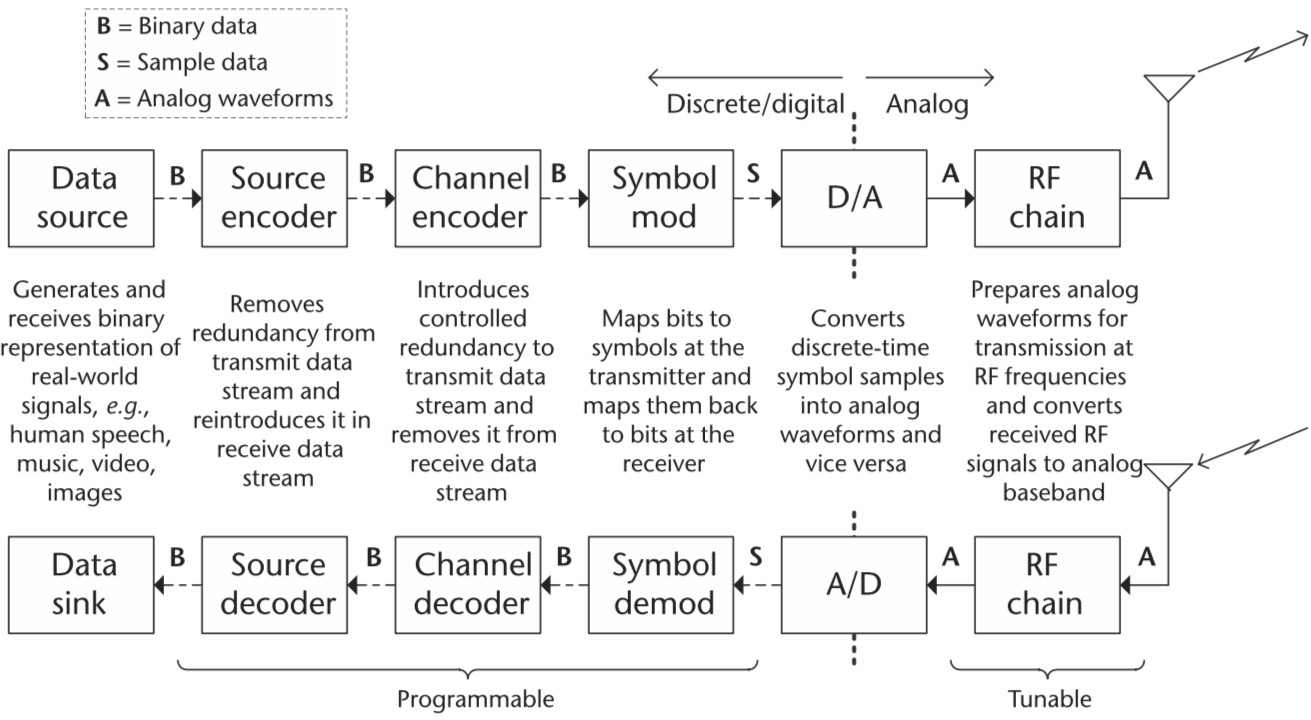
\includegraphics[width=8cm]{forEngineers_SDR_structure}
	\caption{The structure of an SDR}
\end{figure}
In the diagram, the blocks marked as programmable can be implemented in software or programmable logic.\cite{wyglinski2018software}

\section{Software} %Alexander
%GNU Radio Companion
%CubicSDR
%GQRX
%command line tools
%SDR#
%sdrangel
% - Betriebssystem/von wem kommts/Lizenz/Funktionen/Backend
% - Was ist ein Waterfall-Diagramm?

\section{ADS-B}
%Was ist ADS-B
%Wie funktioniert die Codierung?
%Welche Frequenzen gibt es? Welche Antenne wird benötigt?
%Welche Software gibt es/wie funktioniert der Workflow (hackrf_transfer/sox/dump_1090)
%Ergebnisse/Screenshots/flightradar24 Vergleich

\section{NOAA SSTV} %Alexander
%Was ist NOAA
%Wie funktioniert die Codierung?
%Welche Frequenzen gibt es? Welche Antenne wird benötigt?
%Bau der Antenne (verschiedene Typen: V-Dipol, QFH, ...)
%Welche Software gibt es/wie funktioniert der Workflow
%Ergebnisse/Screenshots

\section{replay attack} %Julian
%was ist eine replay attack?
%Beispiel Funksteckdose: Wie funktioniert die Codierung?
%wie funktioniert der workflow? HackRF + hackrf_transfer, parameter, 433 MHz Antenne

%weitere Ideen:
%Radioempfang + Codierung
%rechtliche Lage: ISM-Bänder, Amateurfunklizenz
%LTE
%ship tracking
%Antennentypen: Dipol, Yagi, Patch, Parabol, ...

%\bibliography{references}
%\bibliographystyle{ieeetr}

\end{document}
